\documentclass[11pt]{article}
\usepackage{working-paper,graphicx,booktabs,amsmath}
\newcommand{\RegionHigh}{79.6}
\newcommand{\RegionLow}{12.3}
\newcommand{\WalkGap}{-12.6}
\newcommand{\ServiceGap}{-13.1}
\newcommand{\Sites}{98}
\newcommand{\Points}{98,000}
\newcommand{\Matches}{53,595}
\newcommand{\MatchPct}{54.7}
\newcommand{\Misses}{44,404}
\newcommand{\Errors}{1}
\newcommand{\Selected}{7,185}
\newcommand{\UniquePanos}{7,047}
\newcommand{\NoHit}{16}
\newcommand{\Full}{69}
\newcommand{\Partial}{13}
\newcommand{\PilotPct}{54.5}

\newcommand{\RefPresent}{1,310}
\newcommand{\RefMissing}{39}

\newcommand{\MWPreferredYear}{1,929}
\newcommand{\MWEarlyDates}{2}
\newcommand{\MWImages}{9,997}
\newcommand{\MWImageSites}{82}
\newcommand{\MWInitialImages}{7,184}
\newcommand{\MWReserveImages}{2,813}
\newcommand{\MWSent}{2,594}
\newcommand{\MWUnsent}{7,403}
\newcommand{\MWOccupied}{2,119}
\newcommand{\MWModelEmpty}{475}
\newcommand{\MWHumanReviews}{7}
\newcommand{\MWClassPed}{1,737}
\newcommand{\MWClassRider}{558}
\newcommand{\MWSightings}{6,744}
\newcommand{\MWUnclear}{4,449}
\newcommand{\MWPedPct}{28.8}
\newcommand{\MWRiderPct}{5.4}
\newcommand{\MWUnclearPct}{66.0}

\title{Measuring Women's and Men's Presence on Urban Streets:\\
  Evidence from Google Street View in \Sites{} Cities}
\author{Working paper for discussion}
\date{November 2026}
\begin{document}
\maketitle
\begin{abstract}
Women accounted for \MWPedPct\% of the \MWClassPed{} pedestrian sightings that a vision model classified as women or men in our Google Street View images. Among \MWClassRider{} classified sightings of bicycle, motorcycle, and scooter riders, the share was \MWRiderPct\%. We began by sampling \Points{} locations along mapped streets and walking routes in \Sites{} cities. Google returned a nearby panorama at \MatchPct\% of resolved locations. We acquired \MWImages{} views across \MWImageSites{} cities and screened them for people. Of the \MWSightings{} sightings subsequently counted by the model, \MWUnclearPct\% were too unclear for it to classify. The data document differences in who appears among classifiable sightings and in which streets enter the photographic record. Both matter for interpreting geographic comparisons.
\end{abstract}

\section{Introduction}
Who uses a city's streets, and how does the answer depend on where we look? Travel surveys can establish whether someone left home on a given day. Using Indian time-use diaries, \citet{goel2022mobility} found that among urban residents, women were much less likely than men to report going out. A photograph measures a different aspect of public life. It can record someone working at a stall or waiting for a bus, and a person who spends hours on a street has more chances to appear than someone who crosses it once.

Street photographs give a direct record of who was visible when the camera passed. In a century of archival photographs of Turku, Finland, \citet{turku2021walking} found that women were the most numerous group of pedestrians. In Delhi, \citet{sood2017womencount} reported that men made up about four in five people visible in field photographs. The Delhi study also documented a difficulty that matters for our design: the places fieldworkers photographed departed from the planned sample.

Subsequent work in India allows a closer comparison across cameras. \citet{karekurve2026streetscope} sent fieldworkers with wearable cameras along routes in four cities and counted pedestrians separately from riders. In Delhi, women accounted for 19.8\% of classified adult pedestrian sightings. An independent count in Google Street View imagery from Delhi put the share at 20.0\% \citep{sood2026streetsight}. The estimates are close, although the cameras visited different places at different times. Agreement in Delhi leaves open whether the same sources would give similar estimates in cities where Google photographs fewer streets.

The companion study extended photographic counts to 101 cities using the Global Streetscapes collection of Mapillary and KartaView images \citep{companion,hou}. Contributors chose where to go. Research comparing imagery platforms and examining coverage within cities shows why that choice can affect what a researcher sees \citep{quinn2019every,coverage}. We retain the companion study's pedestrian and rider categories and change the starting point of the sample.

We begin with mapped streets and walking routes in \Sites{} cities and ask where Google Street View supplies a photograph. This lets us measure how often each kind of route enters the photographic record. In the images we acquired, women accounted for \MWPedPct\% of pedestrian sightings classified as women or men and \MWRiderPct\% of classified two-wheeler riders. The evidence has two important limits. A camera on a boulevard may miss people on a parallel footpath, and even in a photographed scene, people in the distance can be too small to classify. We measure coverage separately from classification so that the reader can see where each comparison loses observations.

\section{Data and Research Design}
\subsection{City and street sampling}
The geographic panel draws 75 urban centers uniformly within six regional strata of the \href{https://doi.org/10.2905/1a338be6-7eaf-480c-9664-3a8ade88cbcd}{Global Human Settlement Layer}. The sampling frame contains 11,422 centers. A separate lottery draws 20 of the 101 sites in our earlier imagery study. Five bicycle-study anchors enter with certainty. Overlap yields \Sites{} distinct site polygons. The regional panel supports comparisons of the average urban center in each region. The pooled sample also describes the streets available for comparison with prior fieldwork. A person-weighted or road-length-weighted average across cities would answer a different question.

Within each polygon we drew 1,000 independent positions in proportion to eligible OpenStreetMap route length. A kilometer of eligible footway and a kilometer of residential street receive the same sampling weight. The frame includes ordinary streets, public-facing service roads, pedestrian and shared streets, walking routes, and eligible connectors. Explicit pedestrian restrictions take precedence. An ordinary route with unverified access can enter. Mapped route classification and access may differ from conditions on the ground. Street centerlines generally represent adjacent sidewalks to avoid counting a corridor twice. The frozen November 2026 network also includes routes that may have changed since an older panorama was captured.

We recorded the result of Google's coordinate metadata lookup for every frozen point. A successful response supplies a panorama ID. The lookup supplies one panorama per coordinate. A missing candidate, a request error, an unusable image and an observed image with zero people are distinct outcomes. Persistent server errors receive their own status after retries. The preferred capture year is 2026, with earlier or undated views eligible. Bike comparisons instead use the local fieldwork date and actual route overlap. Capture year alone cannot align time of day or season.

\subsection{Image acquisition and person counts}
We sought up to 100 distinct views per site in the prespecified location order. The initial acquisition yielded \MWInitialImages{} photographs. A second pass cycled through cities with eligible views remaining and added \MWReserveImages{}. Both passes used the original street sample and together produced \MWImages{} photographs in \MWImageSites{} cities. Google lists 2026 as the capture year for \MWPreferredYear{} acquired views. The sample therefore spans several capture periods. We retain the reported dates, including \MWEarlyDates{} views in Phetchaburi labeled August 1970 whose capture dates we could not verify. The panorama lookup and the image download are separate observations: Google can identify a panorama yet fail to return the requested view.

We screened each original $640\times640$ image with the YOLO11s person detector, retaining a view if at least one box had a score of 0.15 or higher. We chose this low threshold because an extra box costs an additional review, whereas a missed person can exclude an occupied street. Muse received the whole photograph for all \MWSent{} qualifying views, including those where the detector had flagged a bystander or a roadside object in error. The \MWUnsent{} views without a qualifying box have detector results only. We do not know how often those views contain people.

We sent each qualifying view to Muse (\texttt{muse-spark-1.3-contributor}) with the companion study's prompt. It counted apparent women and men walking or standing and apparent women and men riding two-wheelers. The pedestrian instructions cover adults and adolescents. They exclude people inside enclosed vehicles and depictions such as posters and statues. A single unclear category includes both pedestrians and riders. The categories record what the model could discern in the image. Each count is linked to the input file and saved response.

\subsection{Outcomes and comparisons}
Our unit is a sighting. A person appearing in two views can contribute twice. For pedestrians, we divide the number classified as women by the number classified as women or men. We calculate the same share separately for riders. A crowded view contributes more sightings than a quiet one. We pool all three city panels for the overall counts and use the regional lottery panel for comparisons across regions. For geographic coverage, we first calculate each city's share of resolved locations with a nearby panorama, then average those shares within each region, giving every selected city equal weight.

\section{Results}
\subsection{Pedestrians and riders}
Muse counted people in \MWOccupied{} views and returned zero in \MWModelEmpty{} others. Women accounted for \MWPedPct\% of classified pedestrian sightings and \MWRiderPct\% of classified rider sightings (Table~\ref{tab:counts}).

\begin{table}[htbp]\centering\small
\caption{Sightings classified by Muse in the reviewed Street View images.}
\label{tab:counts}
\begin{tabular}{lrrrr}
\toprule
Activity & Women & Men & Classified & Women (\%) \\
\midrule
Walking or standing & 500 & 1,237 & 1,737 & 28.8 \\
Riding a two-wheeler & 30 & 528 & 558 & 5.4 \\
\bottomrule
\end{tabular}

\par\smallskip\parbox{.90\linewidth}{\footnotesize The denominator in each row is the number classified as women or men in that activity. Muse also returned \MWUnclear{} unclear sightings. Its response gives no activity breakdown for that category.}
\end{table}

Unclear sightings accounted for \MWUnclearPct\% of the \MWSightings{} sightings that Muse reported. This matters even if every person in the frame is detected. For example, if riders farther from the camera are harder to classify, nearby riders will contribute disproportionately to the reported share. The count of unclear sightings alone tells us neither the size nor the direction of that difference.

Table~\ref{tab:people-region} restricts the comparison to cities drawn in the regional lottery. It shows how many selected cities contributed any photographs and how many contributed a classified pedestrian. In South Asia every selected city contributed classified pedestrians. In sub-Saharan Africa fewer than half did. A pooled share among sightings from those cities cannot describe the cities missing from that row.

\begin{table}[htbp]\centering\small
\caption{Classified pedestrian sightings in the regional city sample.}
\label{tab:people-region}
\begin{tabular}{lrrrrrr}
\toprule
Region & Drawn & Imaged & Classified & Women & Men & Women (\%) \\
\midrule
Americas & 12 & 12 & 11 & 51 & 59 & 46.4 \\
East Asia \& Pacific & 13 & 8 & 7 & 21 & 34 & 38.2 \\
Europe \& Central Asia & 12 & 12 & 9 & 28 & 42 & 40.0 \\
MENA, Afghanistan \& Pakistan & 12 & 8 & 7 & 27 & 108 & 20.0 \\
South Asia & 13 & 13 & 13 & 151 & 427 & 26.1 \\
Sub-Saharan Africa & 13 & 6 & 6 & 44 & 96 & 31.4 \\
\bottomrule
\end{tabular}

\par\smallskip\parbox{.90\linewidth}{\footnotesize Drawn, imaged, and classified are city counts. A classified city contributes at least one pedestrian classified as a woman or a man. Each regional percentage pools those sightings. Cities selected only for overlap with earlier research enter Table~\ref{tab:counts} but are outside this comparison. MENA denotes the Middle East and North Africa.}
\end{table}

\subsection{Coverage by region}
The full lookup returned \Matches{} matches and \Misses{} confirmed misses. The number of lookups still unresolved after retries was \Errors{}. Rate denominators exclude unresolved requests. In the first 100 randomly ordered candidates per site the match rate was \PilotPct\%, compared with \MatchPct\% after checking all points. Across the probability sample, regional averages range from \RegionLow\% to \RegionHigh\%. Figure~\ref{fig:region} shows where those averages conceal differences among cities. In East Asia and the Pacific, sampled cities cluster near zero coverage or in the upper part of the distribution.

\begin{figure}[ht]
\centering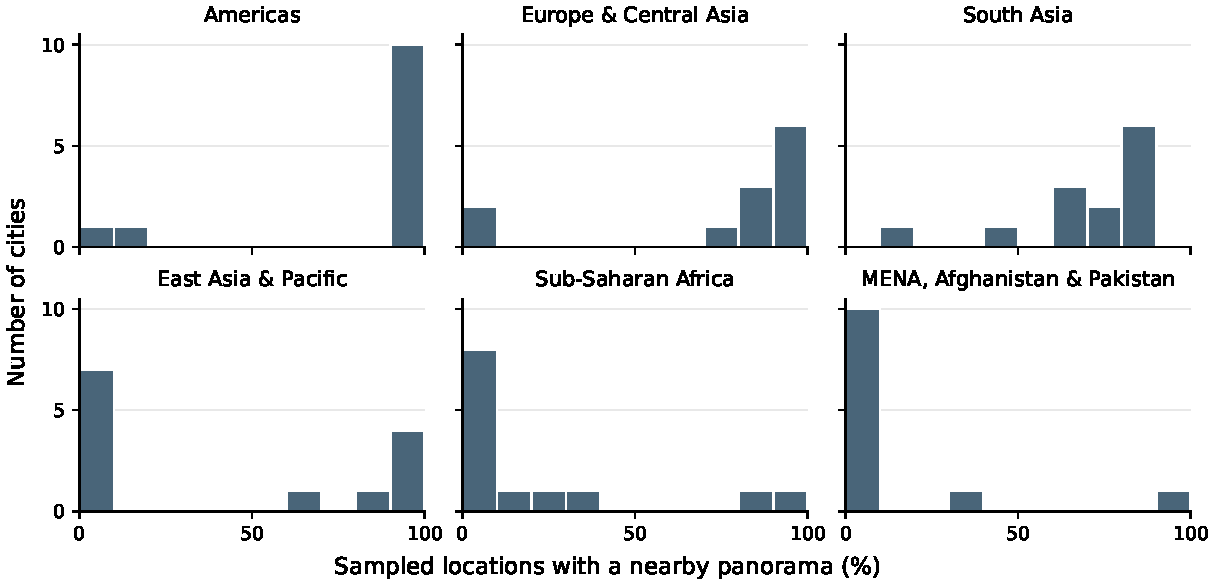
\includegraphics[width=.94\linewidth]{../outputs/google_selection/regional_coverage.pdf}
\caption{Google Street View coverage across the regional probability sample. Each panel counts cities in ten-percentage-point coverage bands. Coverage is the percentage of a city's resolved location lookups that returned a nearby panorama. The scales are the same in every panel.}\label{fig:region}
\end{figure}
\begin{table}[ht]\centering\small
\caption{Estimated coverage of a randomly chosen eligible route position in a randomly chosen urban center, by region.}\begin{tabular}{lrrr}
\toprule
Region & Cities & Mean (\%) & 95\% interval \\
\midrule
MENA, Afghanistan \& Pakistan & 12 & 12.3 & [0.0, 29.1] \\
Sub-Saharan Africa & 13 & 18.9 & [0.0, 38.1] \\
East Asia \& Pacific & 13 & 40.8 & [12.7, 69.0] \\
South Asia & 13 & 70.9 & [58.7, 83.2] \\
Europe \& Central Asia & 12 & 74.7 & [52.2, 97.2] \\
Americas & 12 & 79.6 & [57.4, 100.0] \\
\bottomrule
\end{tabular}

\par\smallskip\parbox{.90\linewidth}{\footnotesize Within each region the city lottery gives every center equal probability. Intervals use the between-city standard error and a Student $t$ critical value. The approximation treats the city sample as drawn with replacement. Intervals are intersected with the feasible range of 0 to 100 percent. MENA denotes the Middle East and North Africa.}\end{table}


\subsection{Coverage by route type}
A pooled comparison mixes differences between cities with differences among streets in the same city. If cities with extensive imagery also map more footpaths, their footpaths can lift the pooled walking-route average. To hold the comparison city constant, we subtract the local ordinary-street match rate from the local match rate for each route family, then average the differences across cities with both types. A city with few connectors counts as much as one with many. The city counts in Table~\ref{tab:routes} show where each comparison has support.
\begin{table}[ht]\centering\small
\caption{Availability by mapped route family in all study sites. The last column gives the mean within-city difference from ordinary streets in percentage points.}\label{tab:routes}
\begin{tabular}{lrrrr}
\toprule
Route family & Points & Matched (\%) & Cities paired & Difference (pp) \\
\midrule
Connector or motorway & 253 & 75.9 & 50 & +12.4 \\
Pedestrian or shared street & 1,994 & 49.2 & 58 & -7.9 \\
Service road & 8,733 & 59.3 & 91 & -13.1 \\
Ordinary street & 80,023 & 52.9 & 98 & +0.0 \\
Walking route & 6,997 & 70.0 & 81 & -12.6 \\
\bottomrule
\end{tabular}
\end{table}

Pooling across cities puts walking routes above ordinary streets in match rate. The order reverses when each walking route is compared with ordinary streets in its own city. The within-city difference averages \WalkGap{} percentage points for walking routes and \ServiceGap{} for service roads. These comparisons describe the frozen sample. They do not show whether the listed street was visible, whether differences reflect mapping practices, or whether Google preferentially photographed streets with more pedestrians. Route verification matters particularly for narrow paths next to major roads. A missing photograph provides no evidence about how many people used the path.

\section{Discussion and Limitations}
\subsection{Streets without imagery}
Let $p$ be the probability that a sampled location has usable imagery. Let $\mu_1$ and $\mu_0$ be the mean number of visible pedestrians under comparable capture conditions at covered and uncovered locations. The target mean is $p\mu_1+(1-p)\mu_0$. Reporting the covered mean alone changes the answer by $(1-p)(\mu_1-\mu_0)$. Our lookup measures the geographic component of $p$. It does not measure $\mu_0$, and even at matched locations image retrieval and human route verification still affect usability.

A comparison with independent photographs can measure part of this gap. We checked a pinned Global Streetscapes catalog for camera positions within 50 meters of each sampled point. The catalog had a nearby camera at \RefMissing{} of the \Misses{} Google misses and \RefPresent{} of the \Matches{} Google matches. Its archived coverage alone cannot support a broad check of missing streets. Camera proximity supplies an upper bound on usable matches to this archive, since a nearby camera can face away from the route. An independent camera survey on a sample of covered and uncovered streets could estimate how much those groups differ. The bike routes provide independent observations where they overlap our locations. Streets missed by both sources would still require field observation or an assumption about who uses them.

\subsection{Detection and classification}
The human protocol asks reviewers to mark individual people on the original image without seeing the model results. At this writing, \MWHumanReviews{} images have a submitted review. That provides too little evidence to estimate the error in the pooled shares. The most informative comparison would include a random sample of detector-negative views alongside positive views. Counting missed pedestrians and riders in the former would show how often screening excludes an occupied scene. Comparing human and Muse counts by category in the latter would show which discrepancies persist after an image reaches the model. Both checks can use the recorded sampling probabilities to account for different review rates.

Women appeared less often than men among the pedestrians and riders whom Muse could classify in these views. Extending that finding to all sampled streets requires evidence about people on uncovered routes, in views the detector skipped, and among sightings the model left unclear. The street sample identifies where to collect the first kind of evidence. The saved images and counts identify where to check the other two.

\bibliographystyle{working-paper-apsr}
\bibliography{refs}
\end{document}
